\documentclass[tikz,border=10pt]{standalone}
\usepackage{tikz}
\usetikzlibrary{positioning}

\tikzset{
  card/.style={draw=blue!70!black, line width=1.2pt, rounded corners=3pt, minimum width=5.4cm, minimum height=4.0cm, align=left, fill=none}
}

\begin{document}
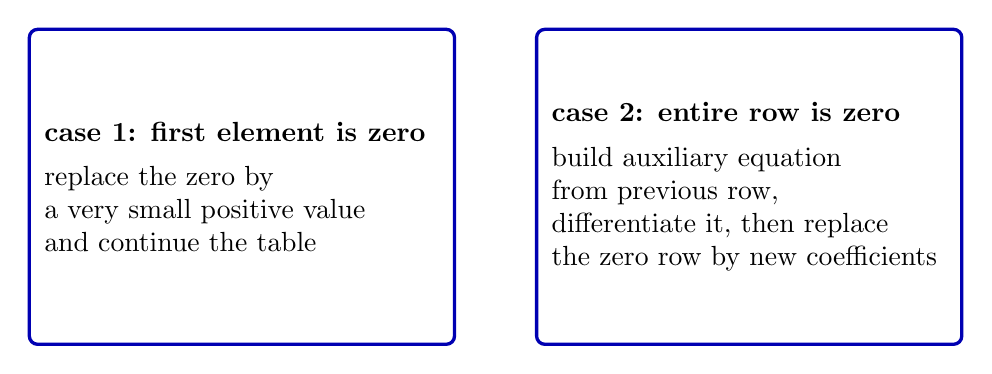
\begin{tikzpicture}[node distance=1.0cm]
  \node[card] (left) {
    \begin{minipage}{4.9cm}
      \textbf{case 1: first element is zero}\\[4pt]
      replace the zero by\\a very small positive value\\and continue the table
    \end{minipage}
  };
  \node[card, right=1.0cm of left] (right) {
    \begin{minipage}{4.9cm}
      \textbf{case 2: entire row is zero}\\[4pt]
      build auxiliary equation\\from previous row,\\differentiate it, then replace\\the zero row by new coefficients
    \end{minipage}
  };
\end{tikzpicture}
\end{document}
